\section{TempCNN}

The article ``Temporal Convolutional Neural Network for the Classification of Satellite Image Time Series'' \cite{tempCNN} presents a machine learning model for classifying satellite image time series data.
The model is based on Convolutional Neural Networks (CNNs) and aims to improve traditional image classification methods by incorporating time series information into the model.

The Temporal Convolutional Neural Network (TempCNN) architecture was used in the following experiments to classify satellite image time series.

The model inputs a series of satellite images and applies a series of convolutional and pooling operations to extract high-level features from the data.
The paper presents a novel approach to classify satellite image time series data and highlights the potential applications of the model in areas such as remote sensing and environmental monitoring.

\subsection{Temporal Convolutions}
Convolutional layers have been proposed as a technique to limit the number of weights a network must learn while exploiting structural dimensions in the data, such as spatial, temporal, or spectral dimensions \cite{NIPS1989_53c3bce6}. 
These layers apply a convolution filter to the output of the previous layer, resulting in an activation map as output, rather than a single activation value per neuron as in dense (fully connected) layers.
For example, with a univariate time series as input, the output of the convolutional layer would be a new time series, with each data point generated by the corresponding convolution filter applied to the original series.

Convolutional layers have the property of sharing their parameters across locations.
This characteristic involves applying the same linear combination by sliding it over the input, resulting in a significant reduction in the number of weights in the layer. 
This reduction is based on the assumption that the same convolution can be beneficial in different parts of the time series.
Therefore, the number of trainable parameters depends only on the filter size of the convolution and the number of units, but not on the input size.

The output size, on the other hand, depends on the input size, the stride, and the padding.
The stride controls the interval between two convolution centers, while padding controls the addition of values (usually zeros) at the beginning and end of the input series before computing the convolution. 
Padding can guarantee that the output is the same size as the input.


\subsection{Model}

The baseline architecture of TempCNN used for the experiments, as shown in Figure \ref{fig:temCNNArchitecture}, consists of three convolutional layers (64 units), one dense layer (256 units), and one softmax layer.
In the experimental section, we will investigate the width (i.e., number of units) of the convolutional layers, the depth (i.e., number of convolutional layers), and the pooling layers of the network.

\begin{figure}[H]
  \centering
  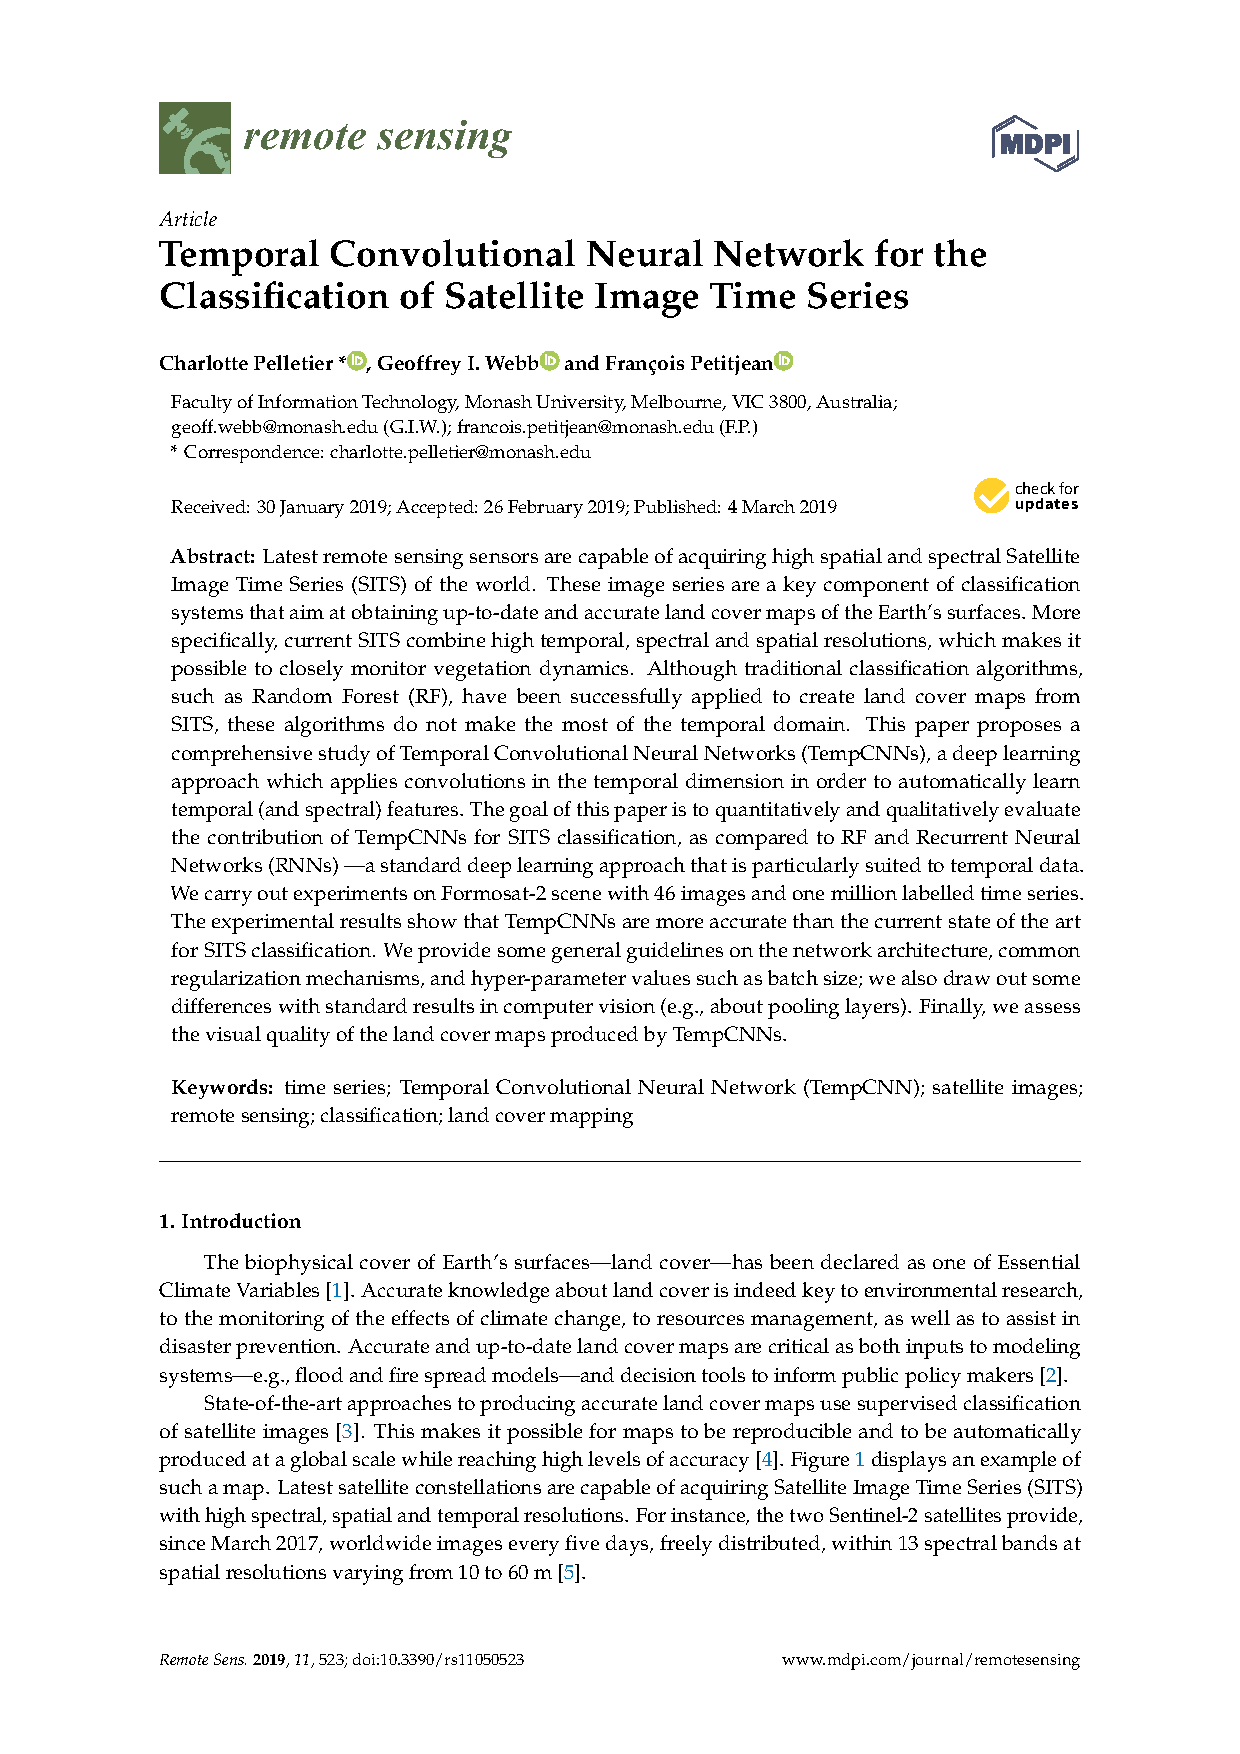
\includegraphics[width=1\textwidth]{tempCNN}
  \caption{Proposed temporal Convolutional Neural Network (TempCNN). The network input is a
  multi-variate time series. Three convolutional filters are consecutively applied, then one dense layer,
  and finally the Softmax layer, that provides the predicting class distribution.    \cite{tempCNN}}
  \label{fig:temCNNArchitecture}
\end{figure}


To prevent overfitting, we employed the same regularization mechanisms described in \cite{tempCNN}:

\begin{itemize}
  \item dropout rate of 0.5 \cite{JMLR:v15:srivastava14a}. 
  \item L2-regularization on the weights (also named weight-decay) applied for all the layers with a small rate of $10^{-6}$ 
  \item batch normalization \cite{DBLP:journals/corr/IoffeS15}.
\end{itemize}

To train the network Adam optimization was used with the standard parameter values: $\beta_1 = 0.9$, $\beta_2 = 0.999$, and $e = 10^{-8}$) \cite{kingma2014adam} 
We used a batch size of 32, and a maximum number of epochs set to 20, with an early stopping mechanism with a patience of zero on the validation loss. 


